\chapter{METODE TUGAS AKHIR}

\section{Alat dan Bahan Tugas Akhir}
Dalam penelitian ini digunakan beberapa perangkat keras dan perangkat lunak. Perangkat keras yang digunakan dalam penelitian ini adalah sebagai berikut
\begin{enumerate}
	\item Apple MacBook Pro dengan prosesor Apple M1 Pro 16-\textit{core} dan memori terpadu 16 GB menggunakan sistem operasi macOS Ventura
	\item STM32 Nucleo-WL55JC1 berbasis ARM Cortex-M0 dan ARM Cortex-M4 sebagai mikrokontroler pada \textit{end-node}
	\item Modul GNSS Teseo-LIV3FL untuk menentukan posisi
	\item Modul Taoglas CGGP.18.2.A.02 sebagai penangkap isyarat GNSS untuk kemudian diolah oleh modul Teseo-LIV3FL
	\item Silicon Labs CP2102 USB \textit{to} TTL \textit{converter} untuk menghubungkan modul Teseo-LIV3FL dengan komputer
	\item \textit{Multimeter} untuk mengukur arus yang digunakan oleh modul Teseo-LIV3FL
	\item Kabel \textit{jumper} untuk purwarupa alat
\end{enumerate}
Selanjutnya, perangkat lunak dan pustaka yang diunakan adalah sebagai berikut
\begin{enumerate}
	\item STM32CubeIDE sebagai IDE untuk mengunggah program ke mikrokontroler STM32 Nucleo-WL55JC1
	\item Aplikasi Teseo-Suite untuk mengunggah konfigurasi dan meninjau konstelasi yang digunakan oleh modul GNSS lebih lanjut
	\item Antares sebagai \textit{platform} untuk menyimpan data yang diterima pada \textit{gateway} LoRaWan
	\item CoolTerm untuk meninjau dan mencatat pembacaan dari \textit{serial port}
\end{enumerate}

\section{Alur Tugas Akhir}
Penelitian ini dilakukan dengan melalui beberapa tahapan. Diagram alir dari tahapan penelitian ini ditunjukan oleh Gambar \ref{Fig: diagram-alir-penelitian}.
\begin{figure}[H]
	\centering
	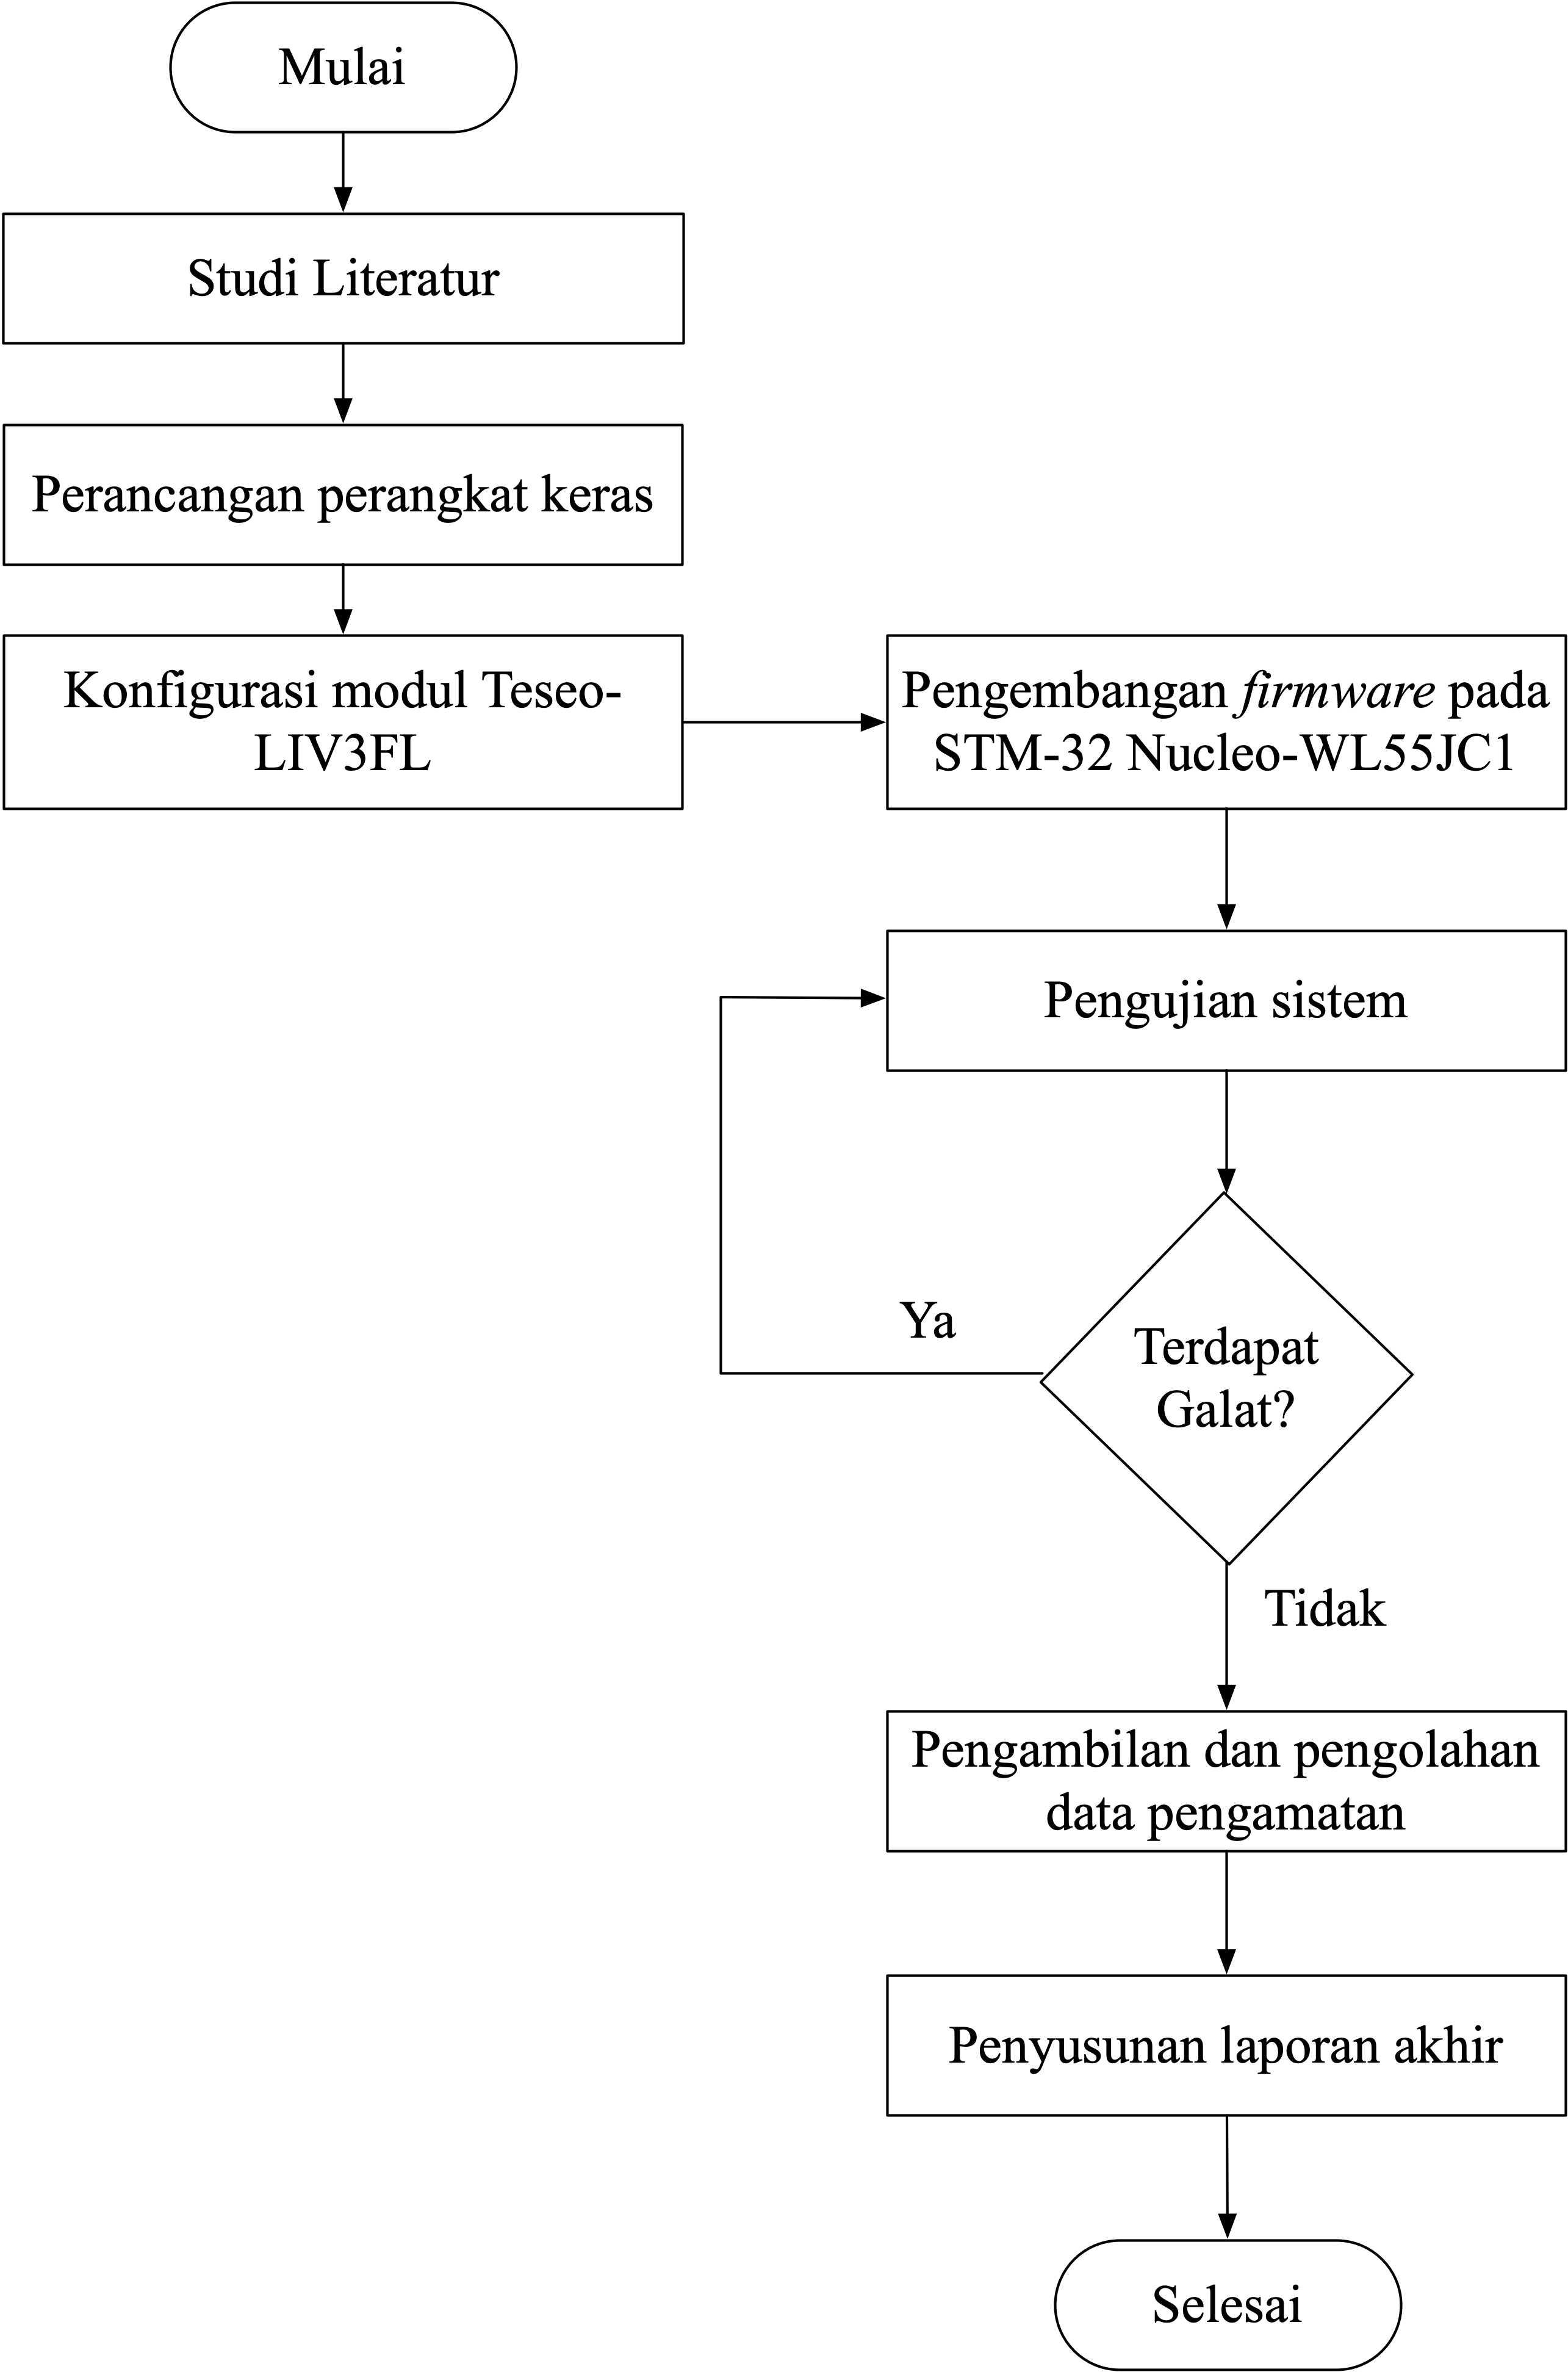
\includegraphics[width=10cm]{contents/chapter-3/diagram-alir-penelitian.png}
	\caption{Diagram Alir Penelitian}
	\label{Fig: diagram-alir-penelitian}
\end{figure}

\section{Studi Literatur}
Studi literatur dilakukan dengan mengumpulkan berbagai materi sebagai acuan dalam melakukan penelitian. Referensi tersebut meliputi artikel dan jurnal ilmiah, laporan penelitian sebelumnya, situs web, dan dokumentasi perangkat yang digunakan. Tahapan ini dilakukan dengan tujuan memperoleh gambaran latar belakang, landasan teori yang digunakan dalam penelitian, dan keahlian	 mengenai topik penelitian.

\section{Persiapan Perangkat Keras dan Perangkat Lunak}
Persiapan perangkat keras yang dibutuhkan adalah pada bagian \textit{end node} saja. Bagian \textit{end node} terdiri dari tiga komponen utama, yaitu antena GNSS, modul GNSS, \textit{tranceiver} LoRaWAN, dan mikrokontroler. Modul GNSS yang digunakan adalah Teseo-LIV3FL dengan antena Taoglas CGGP.18.2.A.02 untuk menerima isyarat dari konstelasi GNSS. Data posisi yang telah diolah oleh modul GNSS dikirimkan dalam format NMEA menggunakan protokol komunikasi UART ke mikrokontroler untuk diolah kembali menjadi data yang siap dikirimkan ke \textit{gateway}. 

Pada aspek perangkat lunak digunakan STM32Cube IDE untuk memrogram mikrokontroler STM32. Selain itu, digunakan \textit{middleware} LoRaWAN dari STMicroelectronics untuk mempermudah konfigurasi LoRaWAN pada mikrokontroler. 

Konfigurasi modul Teseo-LIV3FL dilakukan dengan mengunggah perintah yang diinginkan. Perangkat konversi USB ke TTL digunakan untuk menghubungkan modul ke komputer menggunakan komunikasi UART dengan \textit{baud rate} 9600 Bps. Tangkapan layar dari aplikasi Teseo-Suite Pro ditunjukan oleh Gambar \ref{Fig: teseo-suite}.

\begin{figure}[H]
	\centering
	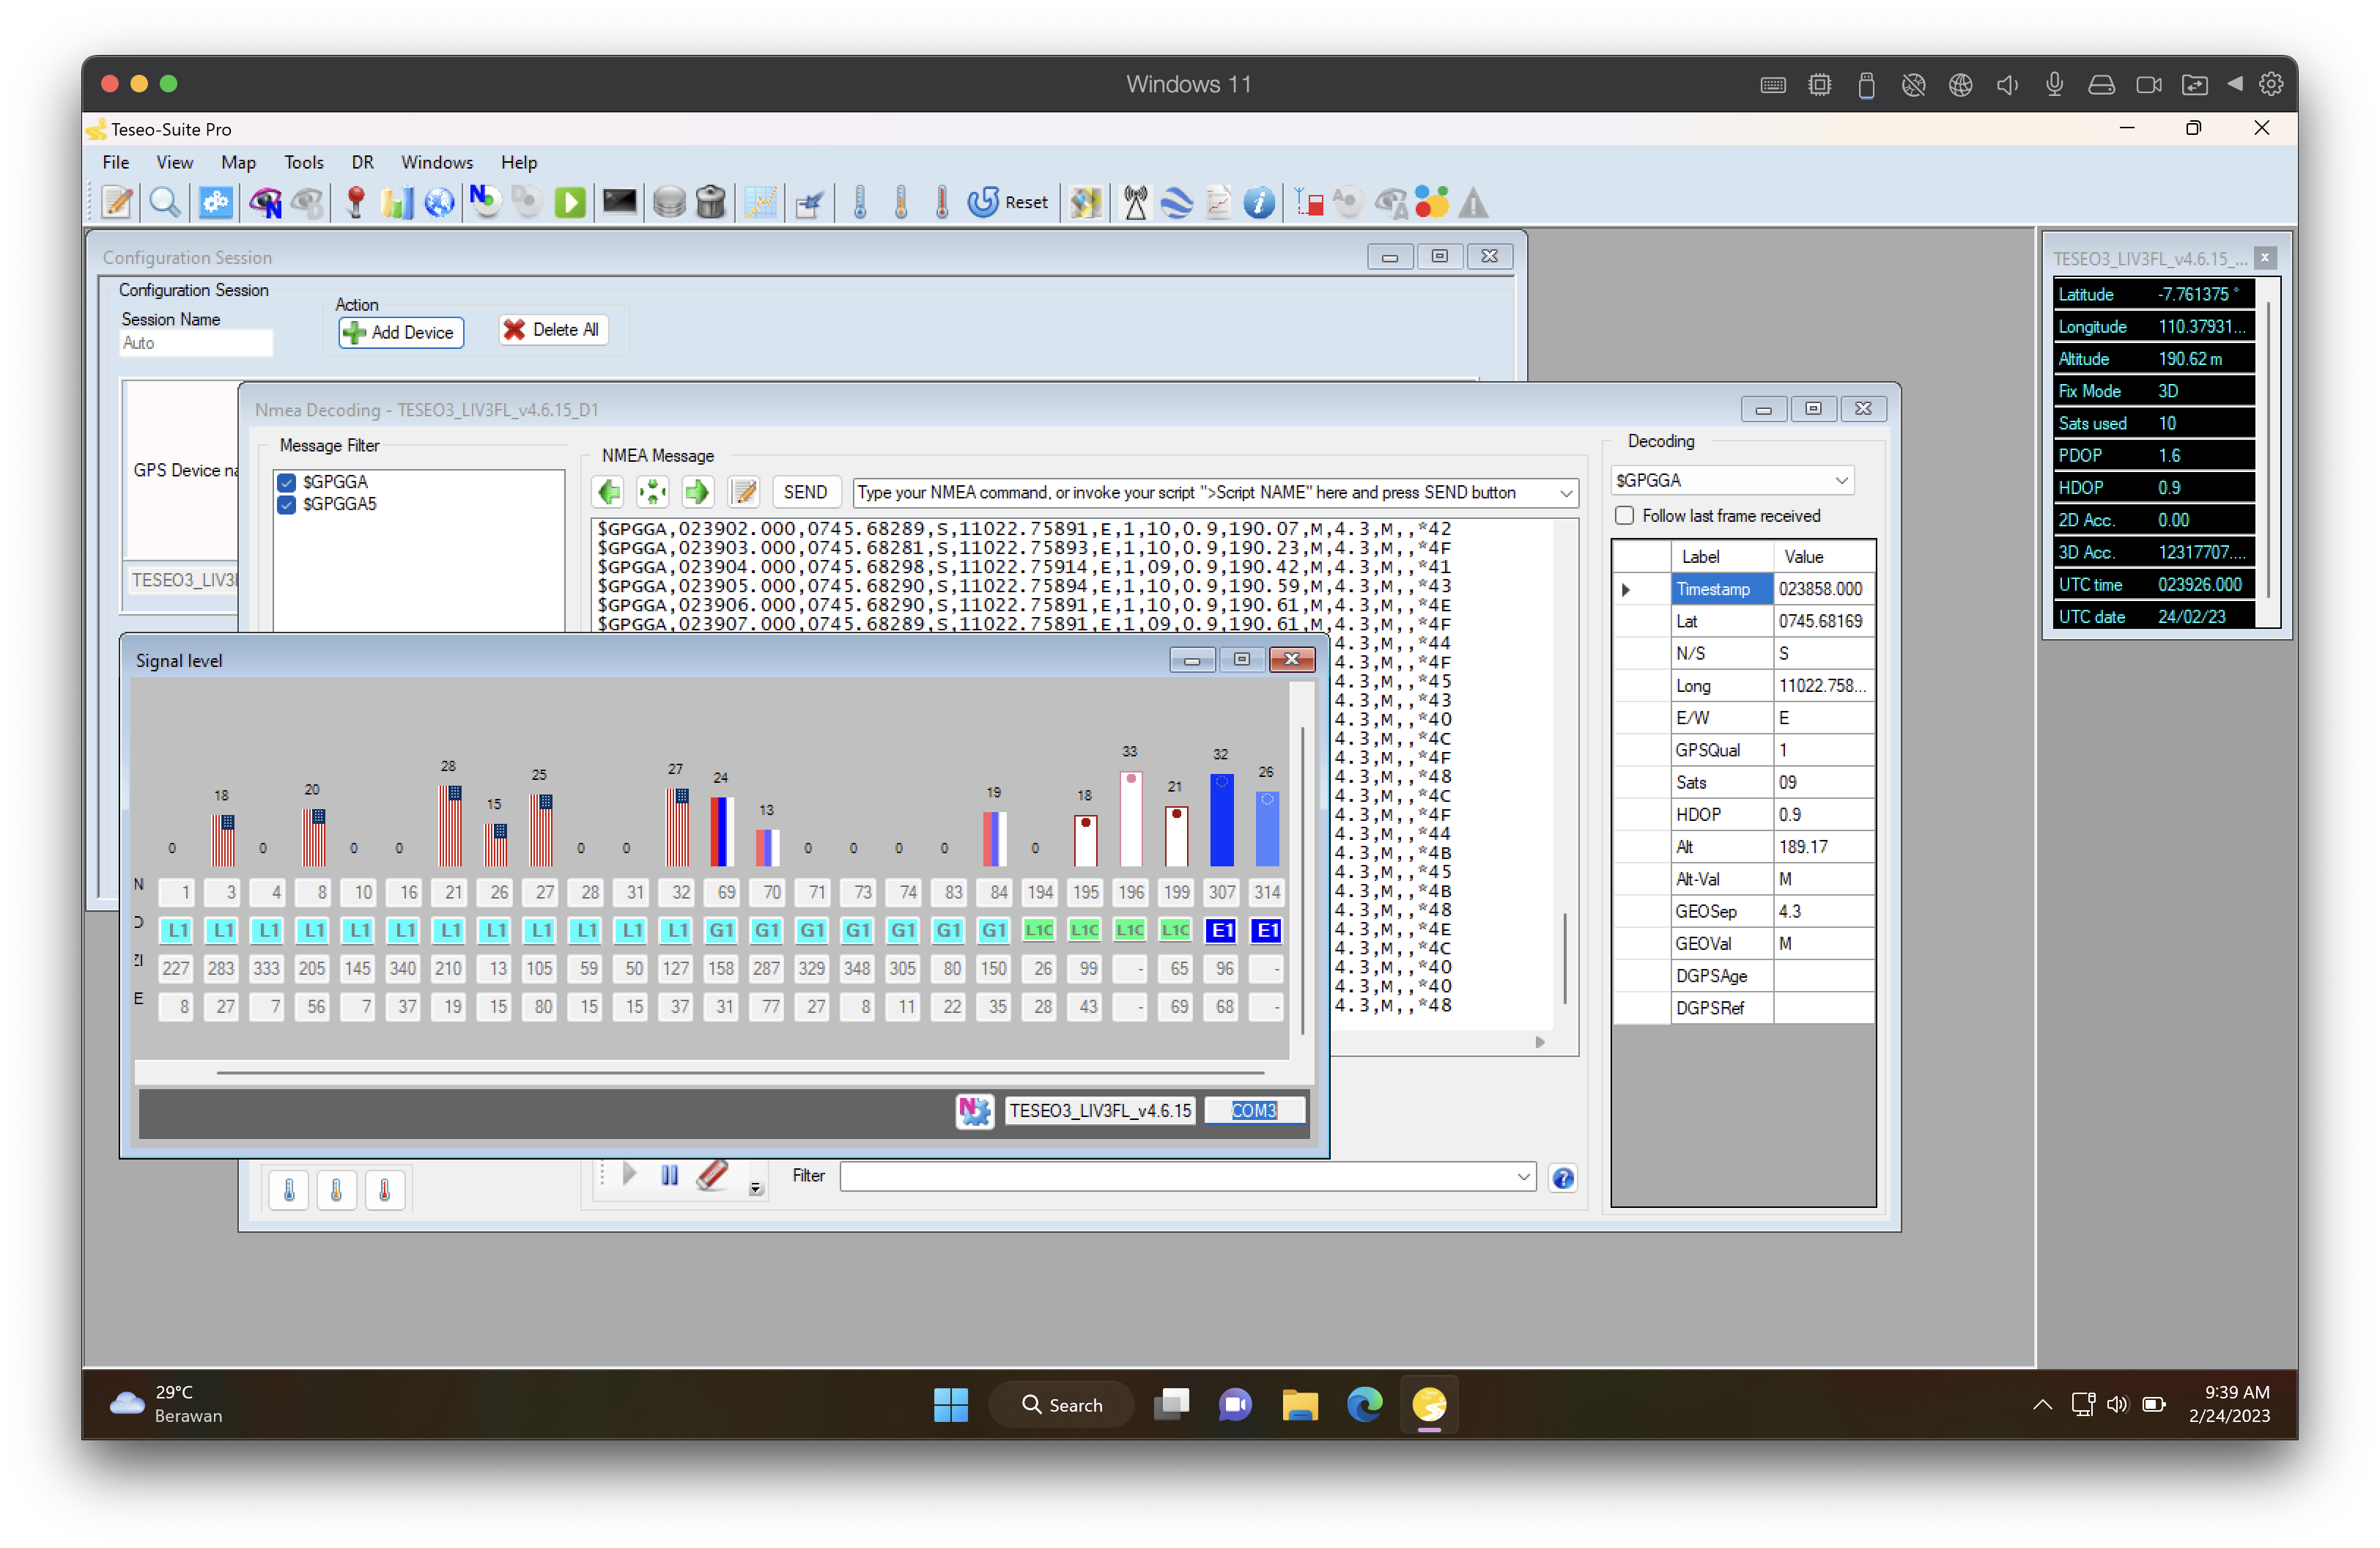
\includegraphics[width=15cm]{contents/chapter-3/teseo-suite.png}
	\caption{Aplikasi Teseo-Suite Pro}
	\label{Fig: teseo-suite}
\end{figure}

Data yang diterima oleh \textit{gateway} kemudian dikirimkan ke \textit{network server} berbasis Chirpstack. \textit{Network server} akan mengolah data mentah dari \textit{gateway} menjadi data yang dapat dimengerti untuk kemudian dikirimkan ke \textit{platform} Antares dengan menggunakan REST API.

\section{Perancangan Sistem}
\begin{figure}[H]
	\centering
	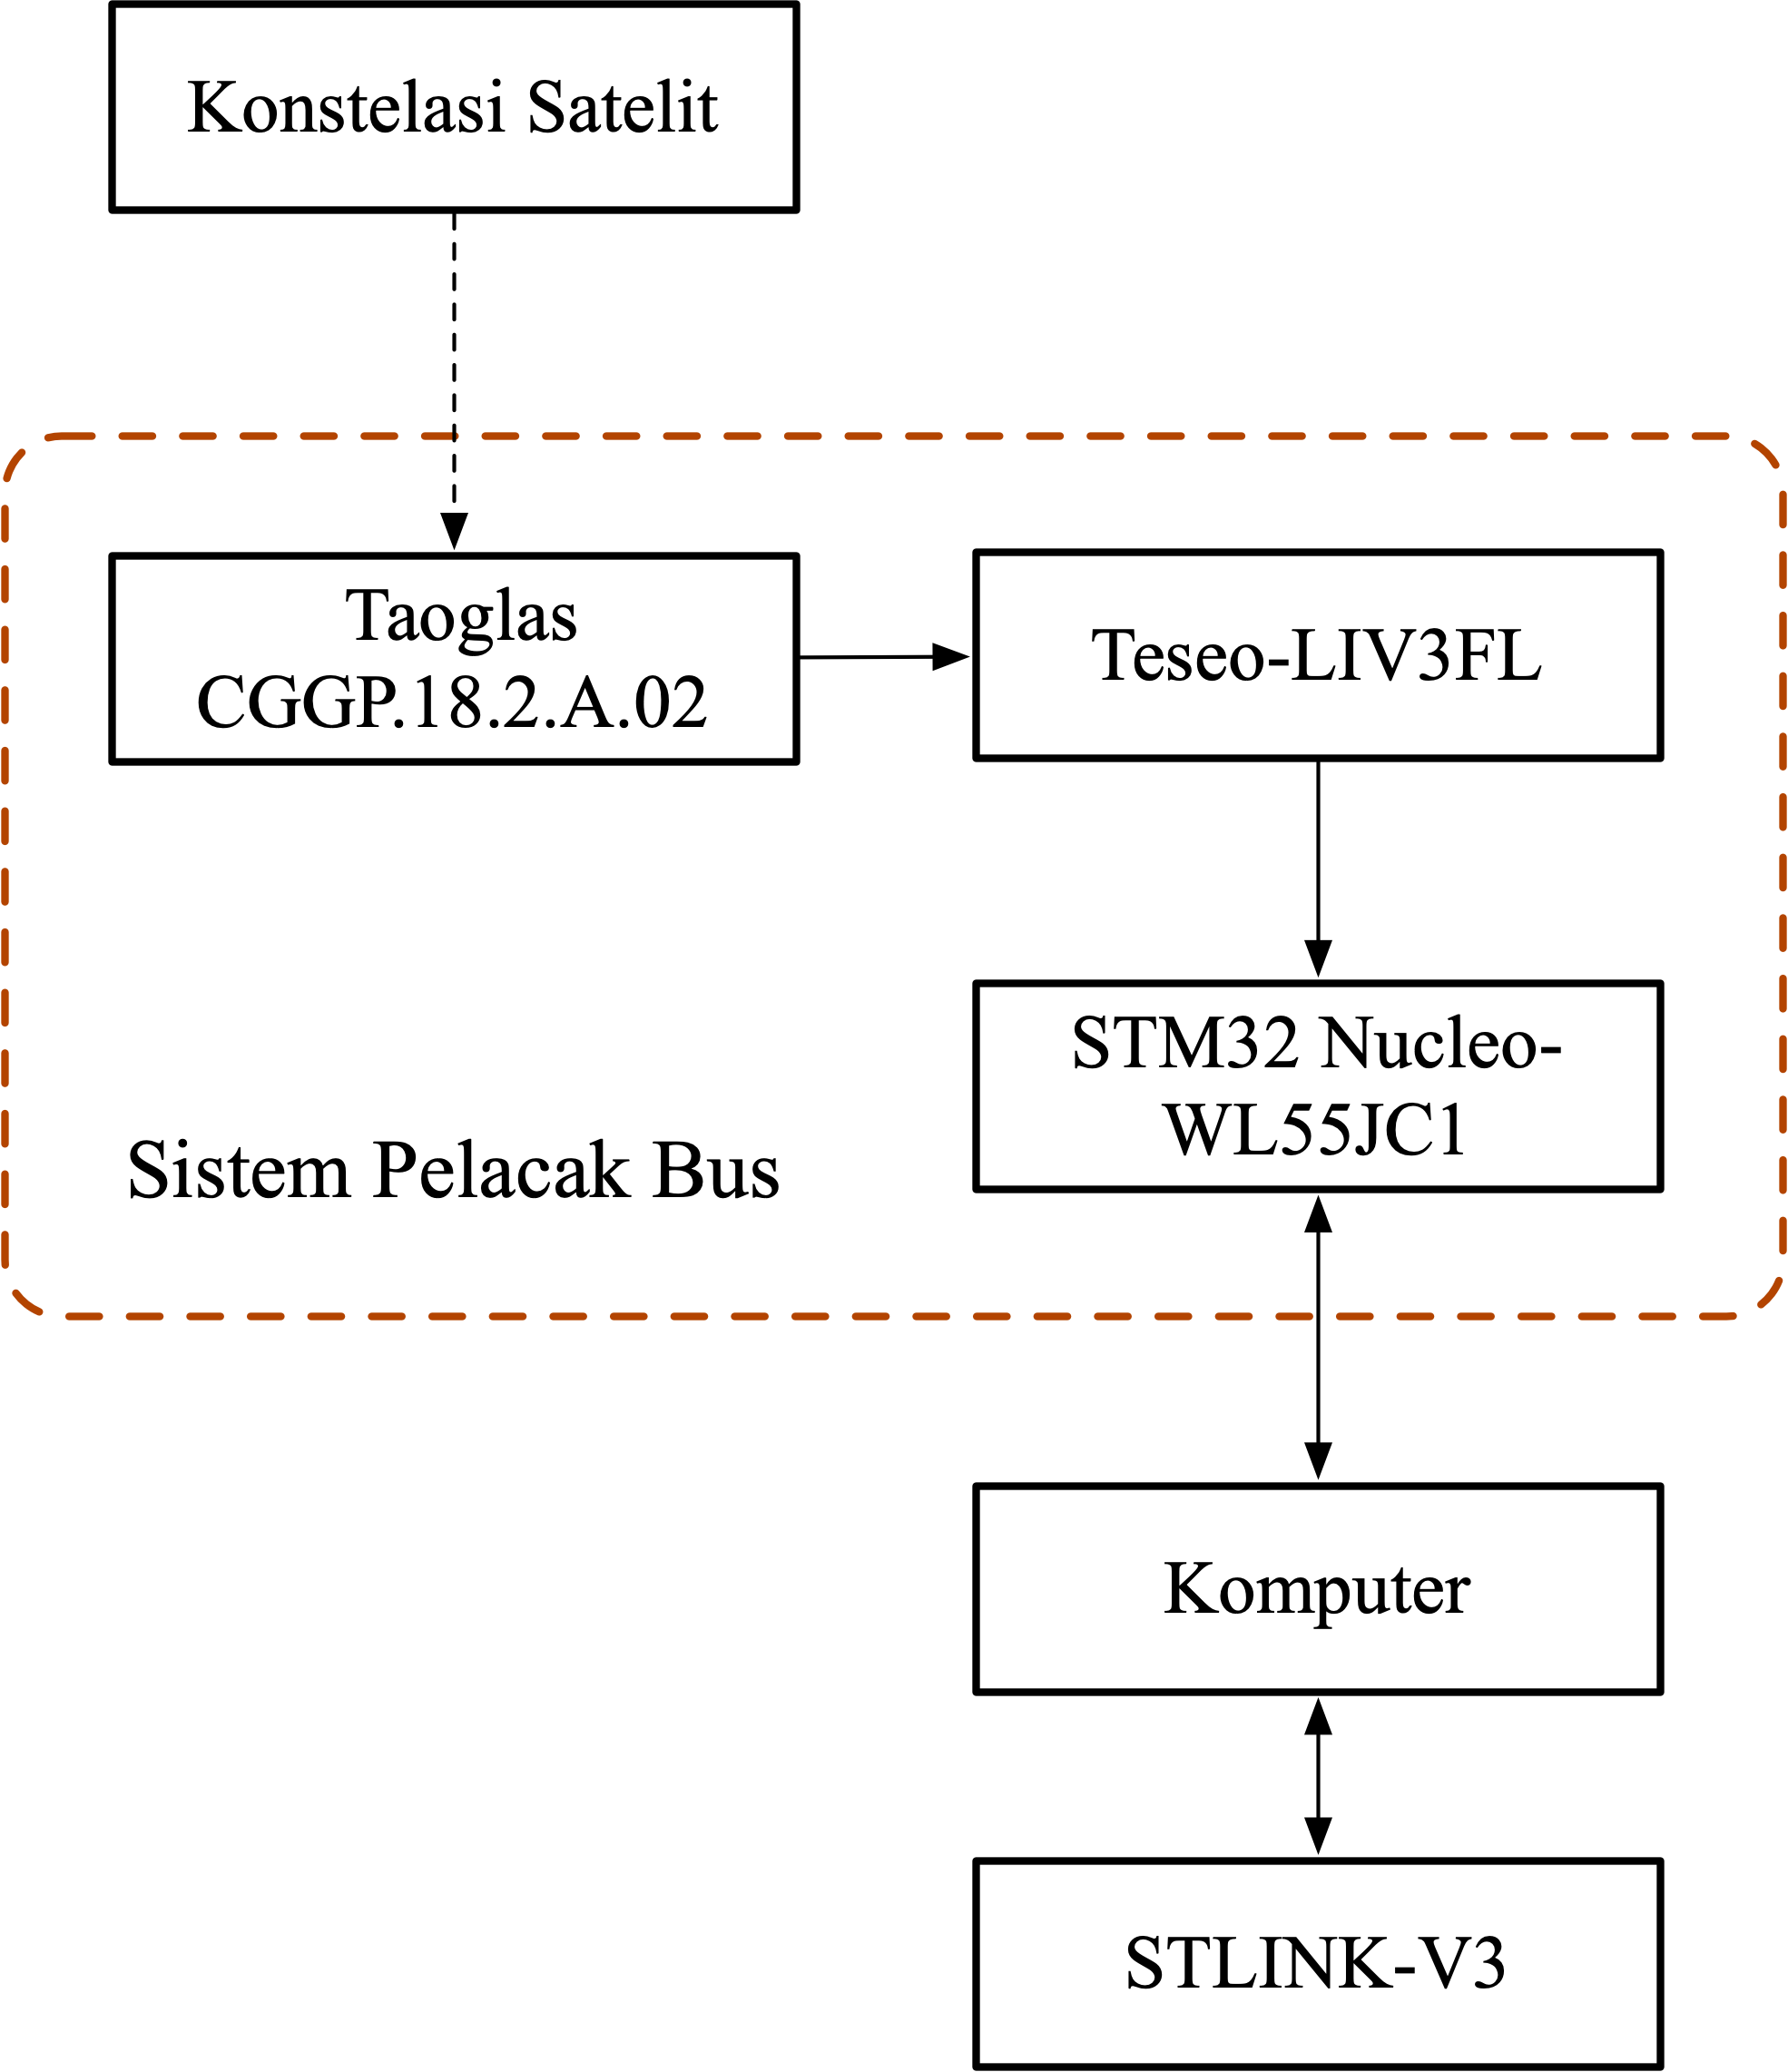
\includegraphics[width=15cm]{contents/chapter-3/system-overview.png}
	\caption{Ikhtisar Sistem}
	\label{Fig: system-overview}
\end{figure}